\subchapter{Bootloader - U-Boot Installing}{Objectives: Install
  the U-Boot bootloader, use basic U-Boot commands}

\section{Installing U-Boot using micro-SD card}

\subsection{Preparing a bootable micro-SD card}

The TI romcode will look for an \code{MLO} ({\em MMC Load})
file in a FAT partition on an SD card. This is precisely what U-Boot
compiled, together with the U-Boot binary (\code{u-boot.img}).

Let's prepare an SD card with such a partition.

Plug the SD card on your workstation. Type the \code{sudo dmesg} command
to see which device is used by your workstation. In case the device is
\code{/dev/mmcblk0}, you will see something like

\begin{verbatim}
[46939.425299] mmc0: new high speed SDHC card at address 0007
[46939.427947] mmcblk0: mmc0:0007 SD16G 14.5 GiB
\end{verbatim}

The device file name may be different (such as \code{/dev/sdb}
if the card reader is connected to a USB bus (either internally
or using a USB card reader).

In the following instructions, we will assume that your SD card is
seen as \code{/dev/sdd}.

Type the \code{mount} command to check your currently mounted
partitions. If SD partitions are mounted, unmount them:

\bashcmd{$ sudo umount /dev/sdd*}

We will erase the existing partition table by simply zero-ing the
first 16 MiB of the SD card:

\bashcmd{$ sudo dd if=/dev/zero of=/dev/sdd bs=1M count=16}

Now, let's use the \code{cfdisk} command to create the first partition
that we need to boot the board:
we are going to use:

\bashcmd{$ sudo cfdisk /dev/sdd}

If \code{cfdisk} asks you to \code{Select a label type}, choose
\code{dos}. This corresponds to traditional partitions tables that DOS/Windows
would understand. \code{gpt} partition tables are needed for disks bigger
than 2 TB.

In the \code{cfdisk} interface, delete existing partitions, then
create only one primary partition, starting from the beginning, with the
following properties:

\begin{itemize}
\item Size: 64MB big
\item Type: \code{W95 FAT32 (LBA)} (\code{c} choice)
\item Bootable flag enabled
\end{itemize}

Press \code{Write} when you are done.

To make sure that partition definitions are reloaded on your
workstation, remove the SD card and insert it again.

Now create a FAT32 filesystem on this new partition:
\footnote{Ubuntu uses version 4.2 of \code{mkfs.vfat} and the FAT
generated by this version of the command is incompatible with what
the TI AM335x romcode expects. Passing the \code{-a} option
is a workaround as described on a
\href{https://bootlin.com/blog/workaround-for-creating-bootable-fat-partition-for-beagle-bone-am335x-on-recent-distros/}
{Bootlin blog post}.}
\begin{bashinput}
$ sudo mkfs.vfat -a -F 32 -n boot /dev/sdd1
\end{bashinput}

You can now make your workstation automatically mount this
partition by removing the SD card and plugging it back. It should
now be mounted on \code{/media/$USER/boot}.

Now, copy the \code{MLO} and \code{u-boot.img} files to the SD card:
\begin{bashinput}
cp MLO u-boot.img /media/$USER/boot1/
sudo umount /media/$USER/boot1/
\end{bashinput}

\subsection{Testing U-Boot}

Insert the SD card in the board slot. To boot the board on the external micro-SD
card, you need to hold the \code{USER} button close to the USB host
port, and then power-up or reset the board. You can then release the
\code{USER} button.

\begin{center}
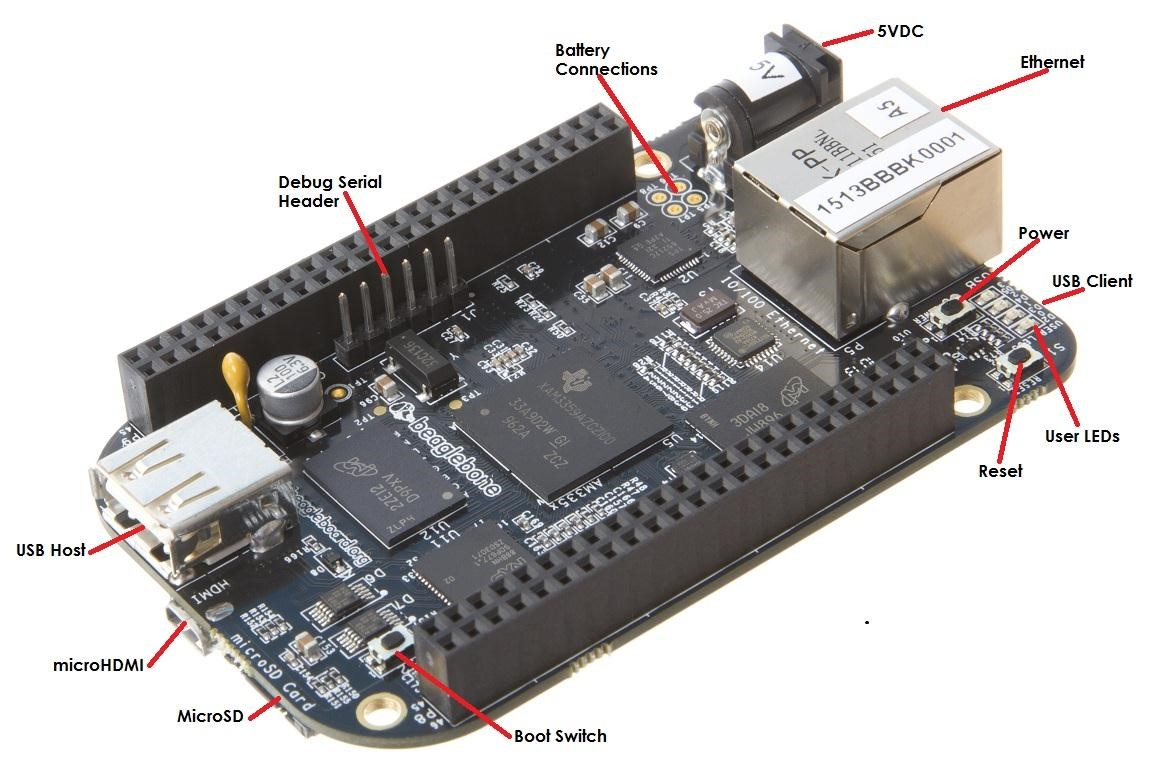
\includegraphics[width=12cm]{labs/u-boot-installing-bbb/bbb-peripheral.png}
\end{center}

The selection of attempting to boot from the external micro-SD card
remains active across resets, until the board is ultimately powered off.

And could use U-Boot on the external micro-SD card to flash a new version of U-Boot
on the internal eMMC. This would allow you to boot without an external micro-SD card.

Here's what you should get on the serial line:

\begin{verbatim}
U-Boot SPL 2024.04-g25049ad560 (Jul 27 2025 - 06:04:45 +0000)
Trying to boot from MMC1


U-Boot 2024.04-g25049ad560 (Jul 27 2025 - 06:04:45 +0000)

CPU  : AM335X-GP rev 2.1
Model: TI AM335x BeagleBone Black
DRAM:  512 MiB
Core:  160 devices, 18 uclasses, devicetree: separate
WDT:   Started wdt@44e35000 with servicing every 1000ms (60s timeout)
NAND:  0 MiB
MMC:   OMAP SD/MMC: 0, OMAP SD/MMC: 1
Loading Environment from FAT... Unable to read "uboot.env" from mmc0:1...
<ethaddr> not set. Validating first E-fuse MAC
Net:   eth2: ethernet@4a100000using musb-hdrc, OUT ep1out IN ep1in STATUS ep2in
MAC de:ad:be:ef:00:01
HOST MAC de:ad:be:ef:00:00
RNDIS ready
, eth3: usb_ether
Hit any key to stop autoboot:  0
=>
\end{verbatim}

Make sure that the version and compile date are right. Otherwise, try
again, because this means that you booted on the internal eMMC.

In U-Boot, type the \code{help} command, and explore the few commands
available.

\section{Installing U-Boot directly to internal eMMC}
TBD

\section{Adding a new command to the U-Boot shell}

Check whether the \code{config} command is available. This command
allows to dump the configuration settings U-Boot was compiled from.

If it's not, go back to U-Boot's configuration and enable it.

\begin{center}
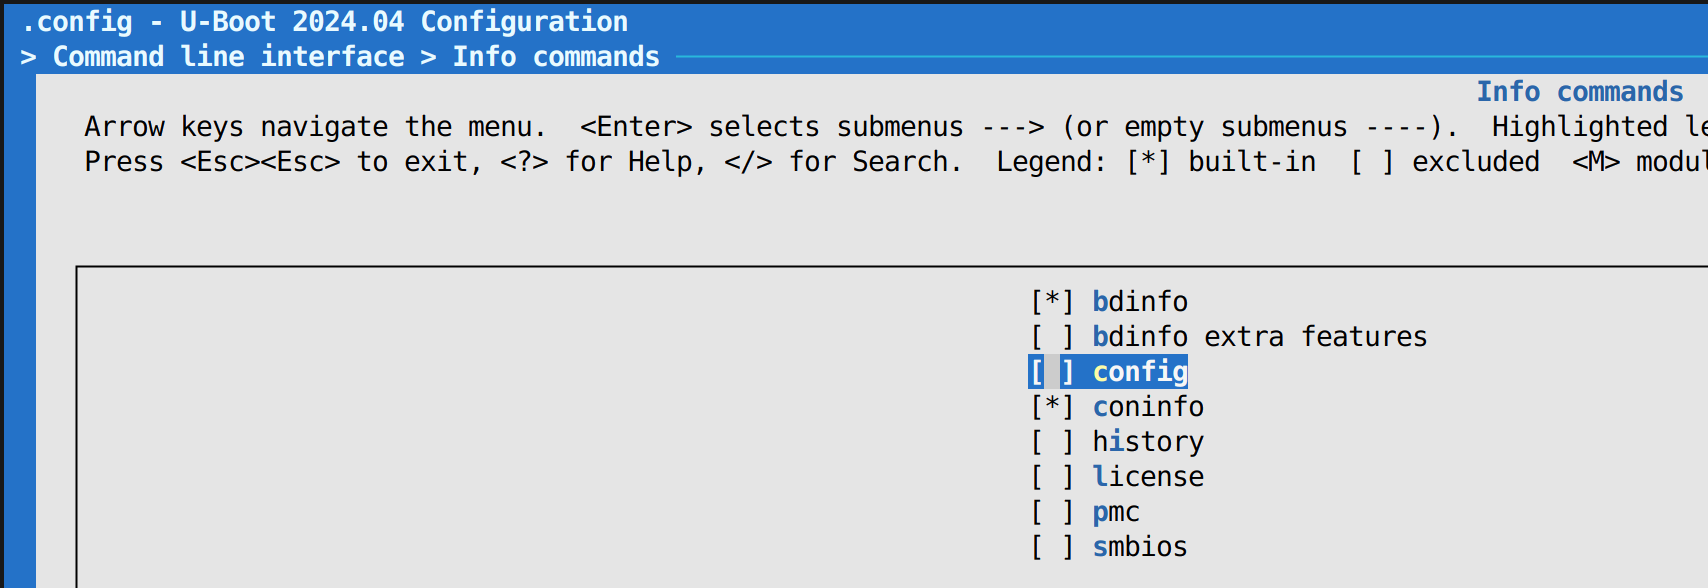
\includegraphics[width=12cm]{labs/u-boot-installing-bbb/enable-config-cmd.png}
\end{center}

Re-run the build of U-Boot, and update the bootloader on the SD card
and test that the command is now available and works as expected.

\section{Playing with the U-Boot environment}

Display the U-Boot environment using \code{printenv}.

Set a new U-Boot variable \code{foo} to a value of your choice, using
\code{setenv}, and verify it has been set. Reset the board, and check
if \code{foo} is still defined: it should not.

Now repeat this process, but before resetting the board, use
\code{saveenv}. After the reset, check the \code{foo} variable is
still defined.

Now reset the environment to its default settings using \code{env
  default -a}, and save these changes using \code{saveenv}.
